\documentclass{sigchi}

\usepackage{balance}       % to better equalize the last page
\usepackage{graphics}      % for EPS, load graphicx instead 
\usepackage[T1]{fontenc}   % for umlauts and other diaeresis
\usepackage{txfonts}
\usepackage{mathptmx}
\usepackage[pdflang={en-US},pdftex]{hyperref}
\usepackage{color}
\usepackage{booktabs}
\usepackage{textcomp}


% Some optional stuff you might like/need.
\usepackage{microtype}        % Improved Tracking and Kerning
% \usepackage[all]{hypcap}    % Fixes bug in hyperref caption linking
\usepackage{ccicons}          % Cite your images correctly!
% \usepackage[utf8]{inputenc} % for a UTF8 editor only


\usepackage{todonotes}
\def\plaintitle{Optical Pumping}
\def\plainauthor{Jung Lin Lee}
\makeatletter
\def\url@leostyle{%
  \@ifundefined{selectfont}{
    \def\UrlFont{\sf}
  }{
    \def\UrlFont{\small\bf\ttfamily}
  }}
\makeatother
\urlstyle{leo}

% To make various LaTeX processors do the right thing with page size.
\def\pprw{8.5in}
\def\pprh{11in}
\special{papersize=\pprw,\pprh}
\setlength{\paperwidth}{\pprw}
\setlength{\paperheight}{\pprh}
\setlength{\pdfpagewidth}{\pprw}
\setlength{\pdfpageheight}{\pprh}

% Make sure hyperref comes last of your loaded packages, to give it a
% fighting chance of not being over-written, since its job is to
% redefine many LaTeX commands.
\definecolor{linkColor}{RGB}{6,125,233}
\hypersetup{%
  pdftitle={\plaintitle},
  pdfauthor={\plainauthor},
  pdfdisplaydoctitle=true, % For Accessibility
  bookmarksnumbered,
  pdfstartview={FitH},
  colorlinks,
  citecolor=black,
  filecolor=black,
  linkcolor=black,
  urlcolor=linkColor,
  breaklinks=true,
  hypertexnames=false
}

% create a shortcut to typeset table headings
% \newcommand\tabhead[1]{\small\textbf{#1}}

% End of preamble. Here it comes the document.
\begin{document}

\title{\plaintitle}

\numberofauthors{1}
\maketitle

\begin{abstract}
%Abstract: This should be a brief (100 words) statement of the experiment (what is it?) and your conclusions (what did you do with it?). Be sure to include your final results, along with their associated errors.
In this lab, we examined whether 
\end{abstract}

\section{Introduction}\label{sec:intro}
\par %Introduction: This should describe the physics and give an overview of what you are going to do. Aim to answer the questions: Why would someone want to do this experiment? What is gained?
Optical pumping is a experimental technique that enable us to measure the ---- splittling levels of Rb atoms in a magnetic field and ---- with degenerate perturbation theory. 
energetically excited to a higher energy state and spontaneous emmision back down to the --- state. Due to the energy splitting of ---- 
\section{Theory}\label{sec:theory}
\par In degenerate perturbation theory of quantum mechanics, we can find the first order corrections to spin orbit coupling and relativistic correction, which together yields the fine structure correction to the eigenstate energies. In addition, there is hyperfine splitting due to interactions of the nucleus of the Rb atom which generates its own electromagnetic fields that gives rise to the perturbation \cite{wiki_hyperfine}.  Additionally, in this experiment, we also apply an external magnetic field (in addition to the Earth's magnetic field) which results in Zeeman splitting in the case of the weak field. In Fig. \ref{splitting}, we can see that the fine structure, hyperfine, and Zeeman interactions splits the energy levels into j , f and $m_f$ levels respectively.
\begin{figure}[h]
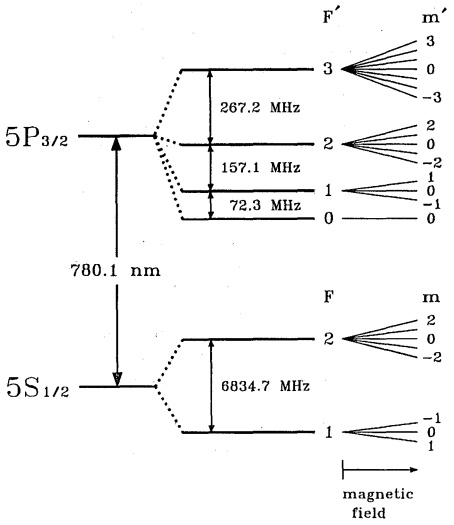
\includegraphics[width=0.45\textwidth]{plots/splitting_diagram.jpeg}
\caption{Energy level splitting of a Rubidium atom. (Source: The Optical Society)}
\label{splitting}
\end{figure}
\begin{equation}\label{currentB}
B_{H} = 0.9\times 10^{-6} \frac{T\cdot m}{A} \frac{N i}{a}
\end{equation}
%Theory: Include the working equations that you will be using but do not include lengthy derivations (such as the Compton or Rutherford formulas) unless specifically asked.where the equations come from and what they are dependent on, (assumptions, conservation laws, etc.), cite reference 
\section{Apparatus and Procedure}\label{sec:ap}
%Apparatus and Procedure: You should have enough detail so that one familiar with physics but not with the particular experiment at hand could reproduce your experiment if necessary. A block diagram of the equipment is essential here—this should be your own, and not copied out of a book or lab manual. Explain the major pieces of equipment and what they do, but do not overwhelm your reader with details here!
We measure the minimum and maximum current value that still yields a symmetric Lissajous curve and make this the error range of our current measurement, since within this range, we can not determine what is the best value corresponding to the resonant frequency. This error is propagated through our subsequent analysis in Sec. \ref{sec:analysis} and to get an error estimate on the final computed value of Earth's magnetic field.
\section{Analysis}\label{sec:analysis}
%Analysis:  the calculations that the lab manual asks you to do are supposed to act as a guide to your analysis, and not as a series of separate calculations. agree with prediction? error analysis? source of error, uncertainty?  
\paragraph{Determining Nuclear Moments of Observed Species}
\par By taking the ratio of the Breit-Rabi equation for the two species: 
\begin{equation*}
\frac{\frac{\nu_1}{B_1} = \frac{2.799}{2I_1+1}}{\frac{\nu_2}{B_2} = \frac{2.799}{2I_2+1}} = \frac{2I_2+1}{2I_1+1}
\end{equation*}
\begin{equation*}
\frac{\nu_1}{\nu_2} = \frac{B_1}{B_2}\Bigg(\frac{2I_2+1}{2I_1+1}\Bigg)
\end{equation*}
We chosing the ``best" value of $\frac{\nu_1}{\nu_2} $ as one and this yielded a 2I+1 ratio of about 2/3. We deduced that if Species 1 was Rb-85 (I=5/2) and Species 2 was Rb-87 (I = 3/2) ~\cite{PhysRev}, then we would get the appropriate 2I+1 ratio. The errors on these deduced values are accurate to 3 significant figures, because we know that nuclear moments must be half-integer values, so the only uncertainty is on the numerical coefficient 2.799. 
\par Knowing the $I_1$ and $I_2$ values, we can use the Breit-Rabi equation to compute the magnetic field and compare this with the one that we obtain from Eq.\ref{currentB}. For species 1, the mean square difference between the two measures of the magnetic field is 0.0915 and for species 2 the mean squared difference is 0.0973. This value gives us an estimate of the systematic error of the possible non-uniformity of the Helmholtz coil number and radius.  Using this technique, we were able to obtain a more accurate estimate of the numerical coefficient in Eq.\ref{currentB} of  $9.963\times 10^{-7}$. 
\paragraph{Data Fitting and Transformation}
\par We perform a linear regression on the data using the model obtained from rearranging the Breit-Rabi equation into the linear form (y = ax+b), where the frequency is the dependent variable and the magnetic field strength is the independent variable.
\begin{figure}[h]
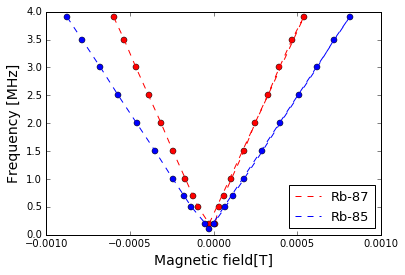
\includegraphics[width=0.45\textwidth]{plots/all_data.png}
\caption{Experimental data of magnetic field strength of Helmholtz coil versus resonant frequency before data transformation.}
\label{linear_fit}
\end{figure}
\par In order to decrease the error on the parameters for linear regression , we flipped the negative data along the x axis so that we could perform two linear fits so that we have double the size of the sample. The error estimates on the parameters can be obtained from the derivation of the  maximum log-likelihood estimator on a linear regression model ~\cite{num_rec}:
\begin{equation}
\sigma_a ^2 = S_{xx}/\bigtriangleup
\sigma_b^2 = S/\bigtriangleup
\end{equation}
where $\bigtriangleup = SS_{xx}-(S_x)^2$,$ S_{xx} = \sum^N_{i=1}\frac{x_i^2}{\sigma_i^2}$, $S_x = \sum^N_{i=1}\frac{x_i}{\sigma_i^2}$, $S =\sum^N_{i=1}\frac{1}{\sigma_i} $.
With this error estimate,  we summarize the fitting coefficients and their respective errors in Table. \ref{fitting_coefficients}.
\begin{table}[]
\centering
\caption{Fitting coefficients on the experimental data, where a is the slope and b is the y-intercept. }
\label{fitting_coefficients}
\begin{tabular}{lllll}
Species & a       & b      & $\sigma_a$ & $\sigma_b$ \\
Rb-85   & 4644.29 & 0.1342 & $1.091\times 10^{-6}$ & 0.231     \\
Rb-87   & 6983.93 & 0.2069 & $1.201\times 10^{-6}$ & 0.573    
\end{tabular}
\end{table}
We obtained a chi squared value of 3.571 for Rb-85 and 3.724 for Rb-87. The chi squared goodness-to-fit test shows that the experimental values are very close to the modelled values (p<0.01) and with the values of nuclear spins found in our analysis.
\begin{figure}[h]
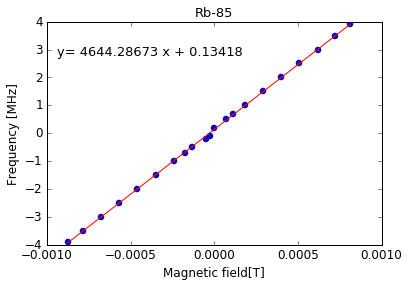
\includegraphics[width=0.45\textwidth]{plots/rb85.png}
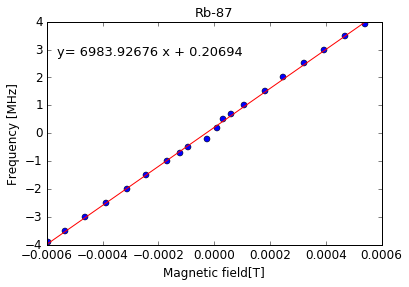
\includegraphics[width=0.45\textwidth]{plots/rb87.png}
\caption{This is the linear regression on the experimental data for Rb-85 and Rb-87. The error bar is too small compared to the pixels spanned by the datapoint, so it can not be seen on this plot.}
\label{linear_fit}
\end{figure}
\paragraph{Estimating Earth's magnetic field}
\par At the zero current point, the magnetic field is zero, so there is no magnetic field contribution from the Helmholtz coil so $B_{total} = B_{earth}$. This could also be thought of as the y intercept of the linear regression: 
$$ B_H = \frac{(2I+1)}{2.799} \nu - B_e $$.
From the two species, we obtained two estimates of the total magnetic field as $59.28\mu$ T for species 1 and $91.428 \mu$ T. The actual magnetic field strength in Berkeley is 48.6$\mu T$,according to Wolfram Alpha. This discrepancy can not be completely accounted for by the error on our recorded measurement. Possible sources error may include instrumentation systematics, non-uniformity of the magnetic field and electronics reading noise. 
\section{Conclusion}\label{sec:conclusion}
%findings, future improvement? 
 
\section*{Acknowledgments}
I am sincerely thankful for support from Professor Harmut Haeffner, Kam-Biu Luk, Don Orlando, and my lab partner Xiyue Wang for contributing to successful completion of this lab.

\bibliographystyle{SIGCHI-Reference-Format}
\bibliography{sample}

%Raw Data: You must include the data that you took in lab in an appendix; the data should be clear enough so that someone could look at it and determine what you measured and how you measured it. You should be keeping a lab notebook, so simply photocopy all relevant pages. Your report should include all of the listed sections, along with the signed Pre-lab and Mid–Lab Discussion sheets.

\end{document}


